\section{Related Work}
\label{sec:Related Work}
This section presents the related work of this thesis. It starts with giving a short overview of several methods used for passive localisation. It shows the projects which use visible light in their localisation schemes. This section finalises by highlighting a paper which attempts to reduce the visible light used in a similar way to this thesis.

\subsection{Passive localisation}
Passive localisation is a hot topic in research and has been tackled by many different research groups in several different ways. The most common method found in literature to detect and track humans is by using Passive Infra-Red (PIR) sensors. These sensors detect the infra-red (heat) radiating from objects and draw conclusions from the observed signals. The passive infrared sensor has been around since 1982 \cite{galvin1982passive} and has been used to detect humans since 1994 \cite{fukuda1994human}.

These days, the research in PIR sensors for detecting and tracking humans focuses in two directions. The first direction is to get more information out of PIR sensors by examining the raw data. M. Waelchli \textit{et al.} for example created a method for estimating the location of a person within the view of the sensor \cite{PIR_Single_Tracking}. The second direction is to track humans with the help of several linked sensors. An example of this, by P. Zappi \textit{et al.} is \cite{PIR_Tracking}. They linked a server to multiple binary human activity sensors, in order to locate and track humans in an indoor building.

Another method for passive localisation, which popped into existence more recently, is developed by M. Youssef \textit{et al.}\cite{WIFI_Tracking}. They created a detect and track application with the help of WIFI access-points (APs), WIFI monitoring-points (MPs) and an application server (AS). The MPs measure the signal strength of the APs, and transmit this data to the AS. The server runs a moving variance algorithm on all of the received signals to detect significant changes in the signal.

Another approach to passive localisation is to use the tiles upon we walk as sensors. This was done by M. Valtonen \textit{et al.} \cite{Tile_Track}. The system measures the capacity between several floor tiles and a receiving electrode. With the help of the measurements, they estimate the position of the person standing on top of the tiles.

\subsection{Passive Visible Light Localisation}
In recent years, a new method for locating and tracking humans has been explored: Passive Visible Light Localisation (PVLL). This method is focussed on using visible light and photo sensors to detect and track humans and objects. Several of these project will be explained briefly, followed by a short comparison between these projects and Dark Sensing.

\subsubsection{Local Light}
Local light, developed by Lascio \textit{et al.}\cite{LocaLight}, is a system which implements passive localization with the help of visible light. The system consists of 3 parts. A light, light sensing RFID tags and a server. The light illuminates the environment. The RFID tags are mounted in the floor, detecting the light produced by the luminaire. The tags transmit their data to a server which processes the data. An overview of the system can be seen in Figure \ref{fig:LocalLight}.

The system works by detecting changes in the light intensity. If the photo diode suddenly senses a huge drop in light, because a shadow is casted on the photo diode by an object or person, the system triggers a detection. The server knows the exact location of all luminaries and photo diodes and is therefore capable to of determining where the object or person is at this moment in time.

\begin{figure}[]
	\centering
	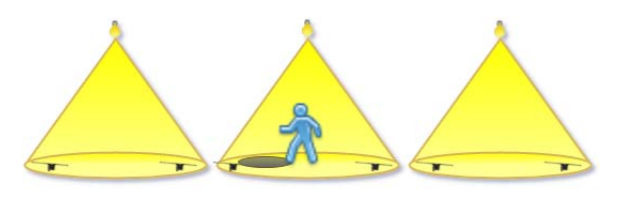
\includegraphics[width=90mm]{pics/LocalLight.png}
	\caption{Overview of the LocalLight system of E.D. Lascio \textit{et al.}\cite{LocaLight}. Lights on the ceiling and light sensing RFID tags on the floor.\label{fig:LocalLight}}
\end{figure}

\subsubsection{Activity sensing using ceiling photo diodes}
Three different projects have been found which have develop a passive localisation scheme using several light/photo diode pairs mounted together on the ceiling. Both take a slightly different approach.

The first project, by J. Zhang \cite{JakesWork}, created a method capable of localising objects on a line between two light/photo diode pairs. By moving an object with three reflective surfaces underneath a light, he managed to localise them at several points on the line by using the specular component of the reflections bouncing of the object. His test set-up can be seen in figure \ref{Zhangpicca}.
\begin{figure}[]
	\centering
	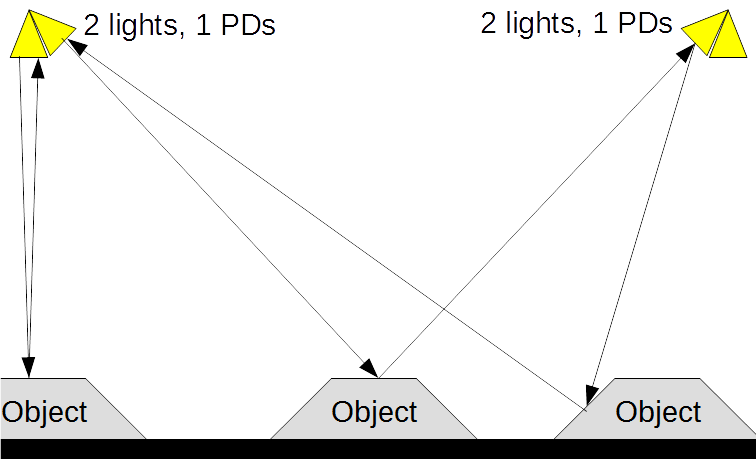
\includegraphics[width=90mm]{pics/Pic_Jake.png}
	\caption{Overview of the system used by J. Zhang \cite{JakesWork}\label{Zhangpicca}}
\end{figure}

The second project, by M. Ibrahim \textit{et al.} \ref{fig:Ceiling_PD}, makes use of modulated lights. Each luminaire transmits light in a different pattern. The photo diode, which is placed next to the light, detects what patterns of light it perceives. If the photo diode does not sense one of the lights it normally does, it triggers a detection as the light was intercepted by a bypassing object. An overview of the set-up can be seen in Figure \ref{fig:Ceiling_PD}/

\begin{figure}[]
	\centering
	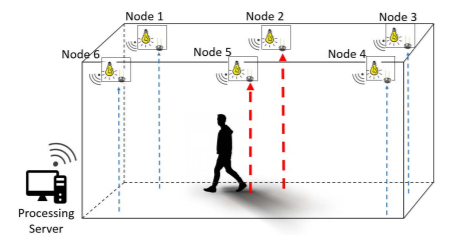
\includegraphics[width=90mm]{pics/lightspdceiling.png}
	\caption{Overview of the system set-up used by M. Ibrahim\cite{Ceiling_PD}. In this specific situation node 2 and 5 detect no light from node 1, because a person is blocking the light.\label{fig:Ceiling_PD}}
\end{figure}

\subsubsection{Comparison with Dark Sensing}
The Dark Sensing project differs from the existing projects in several ways. It's the only project tempting to create a sensing device, only requiring one sensor node instead of multiple and is therefore easier to install and expand. It's also the only project which attempts to save energy. It's also the only project which potentially can be implemented outdoor, mounted on a light post for example, as the other PVLL projects where require either a server in reach of the sensors, or other specific environmental features. Dark Sensing has the potential to be a stand alone product.

The downside of Dark Sensing is that it only focuses on detecting activity. It's therefore unable to track users. All of the other projects are way better in that specific area.

\subsection{Other related projects}
One project that is not related to passive localisation, but inspired us to use short pusles of light is \textit{"The dark light rises"} by Z. Tian \textit{et al.} \cite{Dark_Light_Rises} \cite{Dark_VLC}. This group explores the idea of Visible Light Communication (VLC) with dark light, a VLC primitive that allows light-based communication to be sustained even when LEDs emit extremely-low luminance. The communication works by generating high power, but short light pulses (500ns). These pulses are then used in a pulse position modulation scheme to achieve communication (1.8Kbps at 1.3m) with light while being nearly invisible to the end user. The goals of Dark sensing and Dark VLC are similar: Save light and therefore energy. Both projects however apply this method in different applications.